\documentclass[twoside]{article}
\setlength{\oddsidemargin}{0 in}
\setlength{\evensidemargin}{0 in}
\setlength{\topmargin}{-0.6 in}
\setlength{\textwidth}{6.5 in}
\setlength{\textheight}{8.5 in}
\setlength{\headsep}{0.75 in}
\setlength{\parindent}{0 in}
\setlength{\parskip}{0.1 in}

\usepackage{url}
\usepackage{titlesec}
\setcounter{secnumdepth}{3}
\usepackage{palatino}
\usepackage{marginnote}
\usepackage{multirow}
\usepackage{easybmat,bigdelim,arydshln}
\usepackage[authoryear,round]{natbib}
\usepackage{amssymb,amsmath,amsthm,amsfonts}
\usepackage{mathtools}
%\usepackage{nicematrix}
\usepackage{arydshln}
\usepackage{caption}
\usepackage{hyperref}
\usepackage{tcolorbox}
\tcbuselibrary{skins, breakable, theorems}
\usepackage{newpxtext,newpxmath}
\usepackage{longtable}
\usepackage{enumitem}
\makeatletter

\let\bar\overline

\setlist[itemize]{topsep=0pt,leftmargin=10pt,itemsep=-0.2em}
\usepackage{xcolor}
\usepackage{tikz}
\usepackage{pgfplots}
\pgfplotsset{compat = newest}
\usetikzlibrary{patterns,decorations.pathreplacing,decorations.markings,fit,shapes.geometric,angles,quotes,arrows}
\usepgfplotslibrary{fillbetween}

\usepackage{ifthen}
\usepackage{tikz-3dplot}

\pgfdeclarelayer{ft}
\pgfdeclarelayer{bg}
\pgfsetlayers{bg,main,ft}

\hypersetup{
    colorlinks,
    citecolor=red,
    filecolor=black,
    linkcolor=violet,
    urlcolor=blue
}

\definecolor{myblue}{cmyk}{1,.72,0,.38}
\definecolor{mypurple}{cmyk}{.57,1,0,.58}
\definecolor{myred}{cmyk}{0,.88,.88,.58}
\definecolor{mygreen}{cmyk}{1,0,.69,.66}
\definecolor{myorange}{cmyk}{0,.58,100,.20}
\definecolor{glaucous}{rgb}{0.38, 0.51, 0.71}

\makeatletter
\renewcommand{\thefigure}{\thesection.\arabic{figure}}
\newtheoremstyle{indented}
  {3pt}% space before
  {3pt}% space after
  {\addtolength{\@totalleftmargin}{3.5em}
   \addtolength{\linewidth}{-3.5em}
   \parshape 1 3.5em \linewidth}% body font
  {}% indent
  {\bfseries}% header font
  {.}% punctuation
  {.5em}% after theorem header
  {}% header specification (empty for default)
\makeatother

\newcommand{\ind}{\perp\!\!\!\perp}

\theoremstyle{definition}
\newtheorem{defin}{Definition}[section] % Creates a new counter, number within section
\newtheorem{prt}[defin]{Remark} 
\newtheorem{prts}[defin]{Remarks} % Again share defin's counter
\newtheorem{exmp}[defin]{Example} % etc.
\newtheorem{exmps}[defin]{Examples}
\newtheorem*{note}{Note}
\tcbuselibrary{theorems}

% use counter*=defin to make each tcbtheorem share defin's counter

\newtcbtheorem[use counter*=defin, number within=section]{definition}{Definition}{enhanced, breakable,
    colback = white, colframe = red!55!black, colbacktitle = red!55!black, attach boxed title to top left = {yshift = -2.5mm, xshift = 3mm}, boxed title style = {sharp corners},fonttitle=\bfseries}{def}

\newtcbtheorem[use counter*=defin, number within=section]{theorem}{Theorem}{enhanced, breakable,
    colback = white, colframe = blue!45!black, colbacktitle = blue!45!black, attach boxed title to top left = {yshift = -2.5mm, xshift = 3mm}, boxed title style = {sharp corners},fonttitle=\bfseries}{thm}
    
\newtcbtheorem[use counter*=defin, number within=section]{proposition}{Proposition}{enhanced, breakable,
    colback = white, colframe = teal, colbacktitle = teal, attach boxed title to top left = {yshift = -2.5mm, xshift = 3mm}, boxed title style = {sharp corners},fonttitle=\bfseries}{prop}

\newtcbtheorem[use counter*=defin, number within=section]{lemma}{Lemma}{enhanced, breakable,
    colback = white, colframe = orange!80!black, colbacktitle = orange!80!black, attach boxed title to top left = {yshift = -2.5mm, xshift = 3mm}, boxed title style = {sharp corners},fonttitle=\bfseries}{lemma}

\newtcbtheorem[use counter*=defin, number within=section]{example}{Example}{enhanced, breakable,
    colback = white, colframe = yellow!60!black, colbacktitle = yellow!60!black, attach boxed title to top left = {yshift = -2.5mm, xshift = 3mm}, boxed title style = {sharp corners},fonttitle=\bfseries}{exmp}

\newtcbtheorem[use counter*=defin, number within=section]{assumption}{Assumption}{enhanced, breakable,
    colback = white, colframe = violet!60!white, colbacktitle = violet!60!white, attach boxed title to top left = {yshift = -2.5mm, xshift = 3mm}, boxed title style = {sharp corners},fonttitle=\bfseries}{assump}

\newtcbtheorem[use counter*=defin, number within=section]{algorithm}{Algorithm}{enhanced, breakable,
    colback = white, colframe = green!55!black, colbacktitle = green!55!black, attach boxed title to top left = {yshift = -2.5mm, xshift = 3mm}, boxed title style = {sharp corners},fonttitle=\bfseries}{algm}
%\newtcolorbox{example}[1]{enhanced, breakable, colback = white, colframe = orange!85!black, colbacktitle = orange!85!black, attach boxed title to top left = {yshift = -2.5mm, xshift = 3mm}, boxed title style = {sharp corners},fonttitle=\bfseries, title={Example: #1}}

\newtcbox{\myhl}[1][white]
  {on line, arc = 0pt, outer arc = 0pt,
    colback = #1!20!white, colframe = #1!50!black,
    boxsep = 0pt, left = 1pt, right = 1pt, top = 1pt, bottom = 1pt, boxrule = 0pt, bottomrule =0pt, toprule =0pt}
    
\newtcbox{\myhlrule}[1][white]
  {on line, arc = 0pt, outer arc = 0pt,
    colback = #1!20!white, colframe = #1!50!black,
    boxsep = 0pt, left = 1pt, right = 1pt, top = 1pt, bottom = 1pt, boxrule = 0pt, bottomrule =0.5pt, toprule =0.5pt}
%
% The following commands set up the lecnum (lecture number)
% counter and make various numbering schemes work relative
% to the lecture number.
%
\newcounter{lecnum}
\renewcommand{\thepage}{\thelecnum-\arabic{page}}
\renewcommand{\thesection}{\thelecnum.\arabic{section}}
\renewcommand{\theequation}{\thelecnum.\arabic{equation}}
\renewcommand{\thefigure}{\thelecnum.\arabic{figure}}
\renewcommand{\thetable}{\thelecnum.\arabic{table}}

\newcommand{\sidenotes}[1]{\marginnote{\raggedright\scriptsize#1}}
%
% The following macro is used to generate the header.
%
\newcommand{\lecture}[6]{
   \pagestyle{myheadings}
   \thispagestyle{plain}
   \newpage
   \setcounter{lecnum}{#1}
   \setcounter{page}{1}
   \noindent
   \begin{center}
   \framebox{
      \vbox{\vspace{2mm}
    \hbox to 6.28in { {\bf Econometrics
	\hfill \today} }
       \vspace{4mm}
       \hbox to 6.28in { {\Large \hfill Topic #1: #2  \hfill} }
       \vspace{2mm}
       \hbox to 6.28in { {\it #3 \hfill by #4} }
      \vspace{2mm}}
   }
   \end{center}
   \markboth{Week #1: #2}{Week #1: #2}

   {\bf Key points}: {#5}

   {\bf Disclaimer}: {\it #6}
   \vspace*{4mm}
}
%

\tikzset{-stealth-/.style={decoration={
  markings,
  mark=at position #1 with {\arrow{stealth}}},postaction={decorate}}}

  \tikzset{tangent/.style={
    decoration={
        markings,% switch on markings
        mark=
            at position #1
            with
            {
                \coordinate (tangent point-\pgfkeysvalueof{/pgf/decoration/mark info/sequence number}) at (0pt,0pt);
                \coordinate (tangent unit vector-\pgfkeysvalueof{/pgf/decoration/mark info/sequence number}) at (1,0pt);
                \coordinate (tangent orthogonal unit vector-\pgfkeysvalueof{/pgf/decoration/mark info/sequence number}) at (0pt,1);
            }
    },
    postaction=decorate
},
use tangent/.style={
    shift=(tangent point-#1),
    x=(tangent unit vector-#1),
    y=(tangent orthogonal unit vector-#1)
},
use tangent/.default=1}

\tikzstyle{terminator} = [rectangle, draw, thick, text centered, rounded corners, minimum height=2em]
\tikzstyle{process} = [rectangle, draw, thick, text centered, minimum height=2em]
\tikzstyle{decision} = [diamond, draw, thick, text centered, minimum width=3cm, minimum height=0.5cm]
\tikzstyle{data}=[trapezium, draw, thick, text centered, trapezium left angle=60, trapezium right angle=120, minimum height=2em]
\tikzstyle{arrow} = [thick,->,>=stealth]

\begin{document}
\lecture{11}{Lasso And Beyond: Convex Learning}{}{Sai Zhang}{}{}

\section{Lasso}
Lasso (Least absolute Shrinkage and Selection Operator), proposed by \citet{tibshirani1996regression}, aims to minimize the \myhl[blue!45!black]{\textbf{SSR \textit{(sum of residual squares)}}} subject to the \myhl[red!55!black]{\textbf{$L1-$norm \textit{(sum of the absolute value)}}} of the coefficients being less than a constant.

\subsection{Set up}
For data $\left(\mathbf{x}_i,y_i\right)^n_{i=1}$, where
\begin{itemize}
    \item[-] $y_i$ is the outcome for individual $i$
    \item[-] $\mathbf{x}_i = \left(x_{i1},\cdots,x_{ip}\right)'$ is the $p\times 1$ vector of predictors
\end{itemize}
Then the Lasso estimator $\left(\hat{\alpha},\hat{\boldsymbol{\beta}}\right)$ is defined as 
\begin{align*}
    \left(\hat{\alpha},\hat{\boldsymbol{\beta}}\right) &= \arg\min_{\alpha,\boldsymbol{\beta}}\left\{ \sum^n_{i=1}\left(y_i-\alpha-\sum^p_{j=1}\beta_jx_{ij}\right)^2 \right\} & \text{s.t. }\sum^p_{j=1}\lvert \beta_j \rvert\leq t
\end{align*}

for the $n\times 1$ response vector $\mathbf{y}=\left( y_1,\cdots,y_n \right)'$, the $n\times p$ design matrix $\mathbf{X}=\left(\mathbf{x}_1,\cdots,\mathbf{x}_n\right)'$ where $\mathbf{x}_i= \left( x_{i1},\cdots,x_{ip} \right)' $ is a $p\times 1$ vector. Here $\hat{\alpha}=\bar{y}$, w.l.o.g., let $\bar{y}=0$ and omit $\alpha$ for simplicity.

In matrix form, we have
\begin{itemize}
    \item constrained form:
    \begin{align*}
        \hat{\boldsymbol{\beta}} &= \arg\min_{\boldsymbol{\beta}\in \mathbb{R}^p}\left\{ \frac{1}{2n} \lVert \mathbf{y}-\mathbf{X}\boldsymbol{\beta} \rVert^2_2 \right\} & \text{s.t.\ } & \lVert \boldsymbol{\beta} \rVert_1 \leq t
    \end{align*}
    \item unconstrained form:
    \begin{align*}
        \hat{\boldsymbol{\beta}}(\lambda) &= \arg\min_{\boldsymbol{\beta}\in \mathbb{R}^p}\left\{ \frac{1}{2n} \lVert \mathbf{y}-\mathbf{X}\boldsymbol{\beta} \rVert^2_2 +\lambda \lVert \boldsymbol{\beta} \rVert_1 \right\}
    \end{align*}
\end{itemize}
where the regularization parameter $\lambda \geq 0$:
\begin{itemize}
    \item[-] $\lambda \rightarrow \infty$: $\hat{\boldsymbol{\beta}}_{lasso}=\mathbf{0}$
    \item[-] $\lambda = 0$: $\hat{\boldsymbol{\beta}}_{lasso} \rightarrow\hat{\boldsymbol{\beta}}_{OLS}$
\end{itemize}

\subsection{Solving Lasso}
Lasso is essentially a quadratic optimization problem. Hence, the solution is given by taking the derivative (of the unconstrainted question) and set it equal to 0
\begin{align*}
   && \frac{\mathrm{d}}{\mathrm{d}\boldsymbol{\beta}} \left( \frac{1}{2n} \lVert \mathbf{y}-\mathbf{X}\boldsymbol{\beta} \rVert^2_2 +\lambda \lVert \boldsymbol{\beta} \rVert_1 \right) = 0 \\
   \Rightarrow && \frac{1}{n} \underbrace{\mathbf{X}'}_{p\times n} \underbrace{ \left(\mathbf{y}-\mathbf{X}\boldsymbol{\beta} \right)}_{=\boldsymbol{\epsilon}, n \times 1} &= \lambda \begin{cases}
    \mathrm{sign}\left(\beta_j\right), & \beta_j\neq 0\\
    \left[ -1,1 \right], & \beta_j =0
   \end{cases}
\end{align*}
this result follows the fact the L-1 norm $\lVert \boldsymbol{\beta} \rVert$ is piecewise linear:

\begin{minipage}{0.45\textwidth}
    \centering
        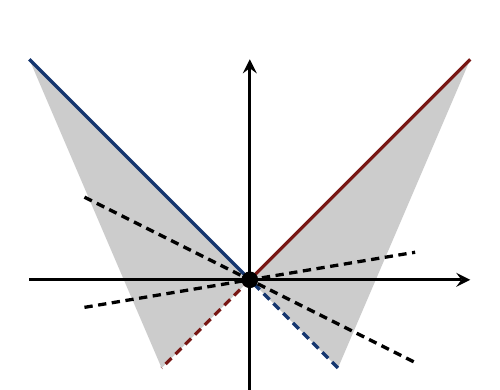
\begin{tikzpicture}[scale=1.4]
            % basics
            \draw [-stealth,color=black,very thick] (2,-1) -- (2,2);
            \draw [-stealth,color=black,very thick] (0,0) -- (4,0);
            \draw [name path = neg_up, color = myblue, very thick] (0,2) -- (2,0);
            \draw [name path = pos_up, color = myred, very thick] (2,0) -- (4,2);
            \draw [name path = pos_down, color = myblue, very thick, densely dashed] (2.8,-0.8) -- (2,0);
            \draw [name path = neg_down, color = myred, very thick, densely dashed] (2,0) -- (1.2,-0.8);
            \filldraw [color=black] (2,0) circle (2pt);
            \draw [color = black, very thick, densely dashed] (0.5,-0.25) -- (3.5,0.25);
            \draw [color = black, very thick, densely dashed] (0.5,0.75) -- (3.5,-0.75);
            \tikzfillbetween[of=neg_up and neg_down, on layer=bg]{black!20!white};
            \tikzfillbetween[of=pos_up and pos_down, on layer=bg]{black!20!white};
        \end{tikzpicture}

        L1-norm (1-dimension)
\end{minipage}
\hfill
\begin{minipage}{0.45\textwidth}
    For each component of the vector of the L-1 norm $f(\beta_j) = \lvert \beta_j \rvert$, we have:
    \begin{itemize}
        \item[-] \textcolor{myred}{$\beta_j>0$: $f'(\beta_j) = 1$}
        \item[-] \textcolor{myblue}{$\beta_j<0$: $f'(\beta_j) = -1$}
        \item[-] $\beta_j=0$: $\mathrm{d}f \in [-1,1]$ (shaded area)
    \end{itemize}
    which gives the results stated above.
\end{minipage}

Take another look at this result 
\begin{proposition}{Lasso Parameter Selection Rule}{lasso-math}
    $$
    \frac{1}{n} \mathbf{X}'  \left(\mathbf{y}-\mathbf{X}\boldsymbol{\beta} \right) =\frac{1}{n} \mathbf{X}'\boldsymbol{\epsilon}  = \lambda \begin{cases}
        \mathrm{sign}\left(\beta_j\right), & \beta_j\neq 0\\
        \left[ -1,1 \right], & \beta_j =0
    \end{cases}
    $$
    which gives a parameter selection criterion: for $\beta_j \neq 0$, \myhl[myred]{$\mathrm{sign}(\beta_j)$ \textbf{must agree} with $\mathrm{Corr}(X_j,\boldsymbol{\epsilon})$}, the correlation between the $j$-th variable $\mathbf{X}_j$ and (full-model) residuals $\boldsymbol{\epsilon}=\mathbf{y}-\mathbf{X}\boldsymbol{\beta}$.
\end{proposition}

\subsection{Algorithm: from LARS to Lasso}
Mathematically, Lasso is quite intuitive, but computionally, it can be quite consuming. \citet{efron2004least} propose an algorithm that takes steps from a all-0 model to the biggest model (OLS), that is, \textbf{Least Angle Regression (LARS)}. 

\subsubsection*{Intuition}
The basic intuition of LARS is quite straight-forward: covariates are considered from the \myhl[myred]{\textbf{\textit{highest}}} corerlation with $\mathbf{y}$ (\textit{smallest} angle from $\mathbf{y}$) to the \myhl[myblue]{\textbf{\textit{least}}} correlated one (\textit{largest} angle from $\mathbf{y}$) (illustrated below).

\begin{figure}[ht]
    \begin{minipage}[b]{0.45\textwidth}
    \centering
      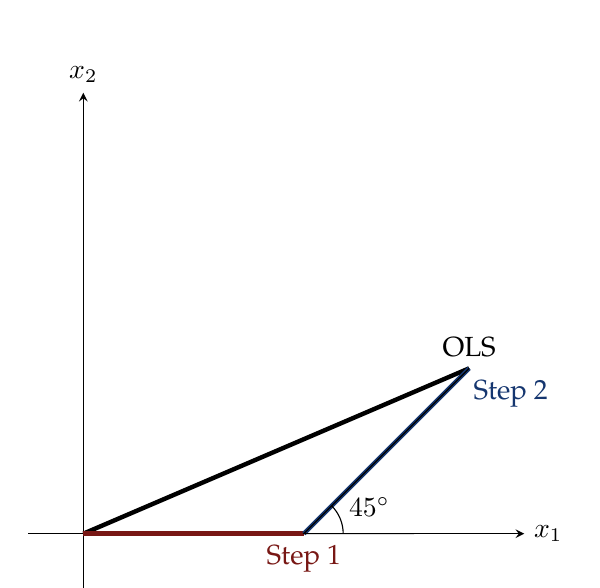
\begin{tikzpicture}[scale=1.4]
          % basics
          \draw [-stealth,color=black,thin] (-0.5,0) -- (4,0) node[right] {$x_1$};
          \draw [-stealth,color=black,thin] (0,-0.5) -- (0,4) node[above] {$x_2$};
          \draw [color=black, ultra thick] (0,0) -- (3.5,1.5) node[above] {OLS};
          \draw [color=myred, ultra thick] (0,0) -- (2,0) node[below] {Step 1};
          \draw [color=myblue, ultra thick] (2,0) -- (3.5,1.5) node[below,xshift=15pt] {Step 2};
          
          \coordinate (X) at (3.5,1.5);
            \coordinate (A) at (2,0);
            \coordinate (Y) at (3,0);

            % Draw Angle
            \draw[thin] (Y) -- (A) -- (X)
            pic ["$45^{\circ}$", draw, thin, angle eccentricity=1.8] {angle = Y--A--X};
      \end{tikzpicture}
    \end{minipage}
    \hfill
    \begin{minipage}[b]{0.45\textwidth}
        \centering
        \tdplotsetmaincoords{60}{45}
        \begin{tikzpicture}
            [scale=5,
                tdplot_main_coords,
                axis/.style={-stealth,black,thin},
                vector/.style={black,very thick},
                LARS/.style={ultra thick}]

            %standard tikz coordinate definition using x, y, z coords
            \coordinate (O) at (0,0,0);
            
            \coordinate (P) at (0.8, 0.6, 0.2);

            \coordinate (P12) at (0.8, 0.6, 0);
            \coordinate (P23) at (0, 0.6, 0.2);
            \coordinate (P13) at (0.8, 0, 0.2);
            \coordinate (P1) at (0.8, 0, 0);
            \coordinate (P2) at (0, 0.6, 0);
            \coordinate (P3) at (0, 0, 0.2);
            
            %draw axes
            \draw[axis] (0,0,0) -- (1,0,0) node[anchor=north east]{$x_1$};
            \draw[axis] (0,0,0) -- (0,1,0) node[anchor=north west]{$x_2$};
            \draw[axis] (0,0,0) -- (0,0,1) node[anchor=south]{$x_3$};

            % projection dash line
            \draw[thin, black, densely dashed] (P12)--(P1);
            \draw[thin, black, densely dashed] (P12)--(P2);
            \draw[thin, black, densely dashed] (P)--(P13);
            \draw[thin, black, densely dashed] (P)--(P23);
            \draw[thin, black, densely dashed] (P23)--(P3);
            \draw[thin, black, densely dashed] (P13)--(P3);
            \draw[thin, black, densely dashed] (P23)--(P2);
            \draw[thin, black, densely dashed] (P13)--(P1);
            \draw[thin, black, densely dashed] (P)--(P12);
            
            %draw a vector from O to P
            \draw[vector] (O) -- (P);

            % draw LARS steps
            \draw[LARS, myred] (O) -- (0.2,0,0) node[left,xshift=-10pt] {Step 1};
            \draw[LARS, myblue] (0.2,0,0) -- (0.6,0.4,0) node[below] {Step 2};
            \draw[LARS, teal] (0.6,0.4,0) -- (P) node[right] {Step 3};

            % approaching, but not exactly reach OLS
            %\draw[thin, teal, densely dashed] (P13)--(0.8,0.35,0.2);
            %\draw[thin, teal, densely dashed] (0.8,0.35,0.2)--(0,0.35,0.2);
        \end{tikzpicture}
    \end{minipage}
\end{figure}

And the steps of the LARS algorithm are
\begin{itemize}
    \item[1] start with the null model $\hat{\boldsymbol{\beta}}=\mathbf{0}$: $\hat{\boldsymbol{\mu}} = \mathbf{X}'\mathbf{0}=\mathbf{0}$ 
    \item[2] calculate residual vector $\mathbf{r} = \mathbf{y}-\hat{\boldsymbol{\mu}}$
    \item[3] determine the correlation vector between $\mathbf{r}$ and each parameter $\mathbf{x}_j,\forall j=1,\cdots,p$: $\mathbf{X}'\mathbf{r}$
    \item[4] pick the largest correlation $\mathbf{x}^*_{\text{step}1,1}$, increase its $\hat{{\beta}}$ to the point where its correlation with $\mathbf{r}$ will be \myhl[red!55!black]{\textbf{equal}} with that of another parameter $\mathbf{x}^*_{\text{step1},2}$ 
    \item[5] next, increase the $\hat{\beta}$ for both $\mathbf{x}^*_{\text{step1},1},\mathbf{x}^*_{\text{step1},2}$ in an \myhl[red!55!black]{\textbf{equiangular}} direction between these two, until a third parameter becomes equally important
\end{itemize}
And keep looping this way, until all the predictors enter the model and eventually $\mathbf{X}'\mathbf{r}=\mathbf{0}$

\subsubsection*{Properties of LARS}
LARS has several properties:
\begin{itemize}
    \item geometrically travels in the direction of \textbf{equal} angle to all active covariates
    \item assume all covariates are independent
    \item computationally quick: only take $m$ steps, where $m$ is the number of parameters being considered
\end{itemize}
And it is in between 2 classic model-selection methods: \textbf{Forward Selection} and \textbf{Stagewise Selection}:
\begin{itemize}
    \item \myhl[red!55!black]{\textbf{Forward Selection}}
    \begin{itemize}
        \item for $\mathbf{y}$, select the most correlated $\mathbf{x}_{j_1}$
        \item regress $\mathbf{x}_{j_1}$ on $\mathbf{y}$, get the residuals
        \item select the most correlated $\mathbf{x}_{j_2}$ with the redisual of $\mathbf{y}$ net of $\mathbf{x}_{j_1}$
    \end{itemize}
    looping this, for a $k-$parameter linear model, it takes $k$ steps. Forward Selection is an aggressive fitting technique, can be overly greedy (some important predictors may be eliminated due to correlation with already selected variables).
    \item \myhl[red!55!black]{\textbf{Forward Stagewise}}
    \begin{itemize}
        \item also begin with $\hat{\boldsymbol{\mu}}=0$
        \item for a current Stagewise estimate $\hat{\boldsymbol{\mu}}$, the current residual vector is then $\mathbf{y}-\hat{\boldsymbol{\mu}}$, its correlation with $\mathbf{X}$ is then  $\mathbf{X'}(\mathbf{y}-\hat{\boldsymbol{\mu}})\equiv \hat{\mathbf{c}}$
        \item next, heavily computational, go in the direction of the greatest current correlation, but by only a \myhl[red!55!black]{\textbf{small}} step $$ \hat{j}= \arg\max\lvert \hat{c}_j \rvert, \ \hat{\boldsymbol{\mu}}\rightarrow \hat{\boldsymbol{\mu}}+\epsilon\cdot \mathrm{sign}(\hat{c}_{\hat{j}})\cdot \mathbf{x}_{\hat{j}} $$
    \end{itemize}
\end{itemize}

\section{Penalized Least Square Estimation}
Lasso is one special class of Penalized Least Square (PLS) Estimation. For the linear regression model $\mathbf{y}=\mathbf{X}\boldsymbol{\beta}+\boldsymbol{\epsilon}$, if $\boldsymbol{\epsilon} \sim \mathcal{N}(\mathbf{0},\sigma^2 \mathbf{I}_n)$, we have PLS as
$$
\min_{\boldsymbol{\beta}\in \mathbb{R}^p}\left\{ \frac{1}{2n} \lVert \mathbf{y}-\mathbf{X}\boldsymbol{\beta} \rVert^2_2 + \sum^p_{j=1}p_{\lambda}\left( \lvert \beta_j \rvert \right) \right\}
$$
where $p_{\lambda}(\cdot)$ is a penalty function indexed by the regularization parameter $\lambda \geq 0$. \citet{antoniadis2001regularization} showed that the PLS estimator $\hat{\boldsymbol{\beta}}$ has the following properties:
\begin{itemize}
    \item \textbf{\underline{sparsity}}: if $\min_{t\geq 0}\left\{ t+p'_{\lambda}(t) \right\}>0$
    \item \textbf{\underline{approximate unbiasedness}}: if $p'_{\lambda}(t)=0$ for $t$ large enough
    \item \textbf{\underline{continuity}}: iff $\arg \min_{t\geq 0}\left\{ t+p'_{\lambda}(t) \right\}=0$
\end{itemize}
In general
\begin{itemize}
    \item[-] the \myhl[red!55!black]{\textbf{sigularity}} of penalty function at the origin, $p'_{\lambda}(0_+)>0$ is needed for generating \textbf{sparsity} in variable selection
    \item[-] the \myhl[red!55!black]{\textbf{concavity}} is needed to reduce the bias
\end{itemize}


\begin{figure}[ht]
    \centering
    \begin{minipage}[b]{0.45\textwidth}
    \centering
      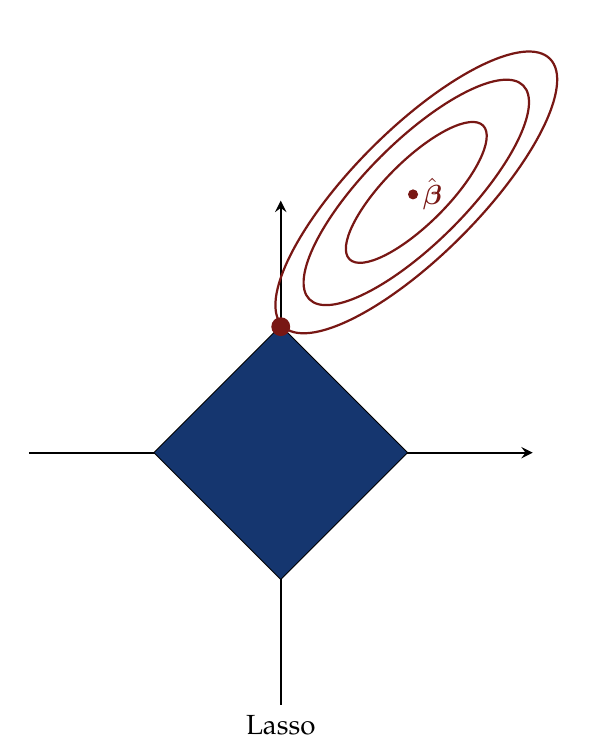
\begin{tikzpicture}[scale=1.6]
          % basics
          \draw [-stealth,color=black,thick] (0,2) -- (4,2);
          \draw [-stealth,color=black,thick] (2,0) node[below] {Lasso} -- (2,4);
          \draw [name path=lup,color=black,thick] (1,2) -- (2,3) -- (3,2);
          \draw [name path=ldown,color=black,thick]  (3,2) -- (2,1) -- (1,2);
          \draw [name path=lmid, color=black, thick] (1,2) -- (3,2);
          \tikzfillbetween[of=lup and ldown, on layer=main]{myblue};
          \draw [rotate=45, thick, color=myred] (5.05,0.7) ellipse (1.5cm and 0.5cm);
          \draw [rotate=45, thick, color=myred] (5.05,0.7) ellipse (1.2cm and 0.4cm);
          \draw [rotate=45, thick, color=myred] (5.05,0.7) ellipse (0.75cm and 0.25cm);
          \filldraw [color=myred] (3.05,4.05) circle (1pt) node[right] {$\hat{\boldsymbol{\beta}}$};
          \filldraw [color=myred] (2,3) circle (2pt);
      \end{tikzpicture}
    \end{minipage}
    \hfill
    \begin{minipage}[b]{0.45\textwidth}
        \centering
        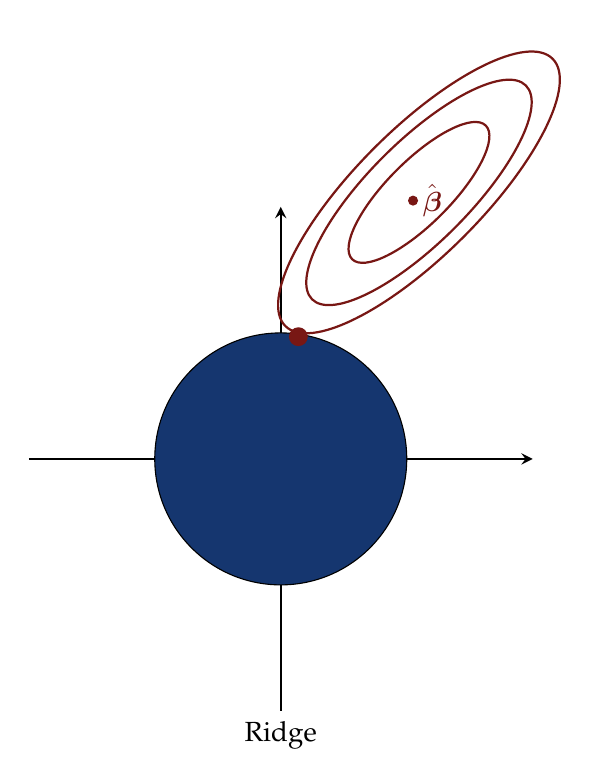
\begin{tikzpicture}[scale=1.6]
            % basics
            \draw [-stealth,color=black,thick] (0,2) -- (4,2);
            \draw [-stealth,color=black,thick] (2,0) node[below] {Ridge} -- (2,4);
            \draw [color=black,thick] (2,2) -- (2,1);
            %\draw [name path=ldown,color=black,thick]  (3,2) -- (2,1) node[right,xshift=2pt, yshift=-2pt] {Lasso} -- (1,2);
            %\draw [name path=lmid, color=black, thick] (1,2) -- (3,2);
            \node[circle,draw,minimum size=3.2cm, fill =myblue] (c) at (2,2){};
            \draw [rotate=45, thick, color=myred] (5.1,0.72) ellipse (1.5cm and 0.5cm);
            \draw [rotate=45, thick, color=myred] (5.1,0.72) ellipse (1.2cm and 0.4cm);
            \draw [rotate=45, thick, color=myred] (5.1,0.72) ellipse (0.75cm and 0.25cm);
            \filldraw [color=myred] (3.05,4.05) circle (1pt) node[right] {$\hat{\boldsymbol{\beta}}$};
            \filldraw [color=myred] (2.14,2.97) circle (2pt);
        \end{tikzpicture}
    \end{minipage}
\end{figure}

\newpage
\bibliographystyle{plainnat}
\bibliography{ref.bib}

\end{document}